\documentclass{wissdoc}
% Autor: Roland Bless 1996-2009, bless <at> kit.edu
% ----------------------------------------------------------------
% Diplomarbeit - Hauptdokument
% ----------------------------------------------------------------
%%
%% $Id: thesis.tex 65 2012-05-10 10:32:11Z bless $
%%
%
% Zum Erstellen zweiseitiger PDFs (für Buchdruck) in der Datei "wissdoc.cls" folgende Zeile abändern:
%
% \LoadClass[a4paper,12pt,oneside]{book} % diese Klasse basiert auf ``book''
% in
%\LoadClass[a4paper,12pt,titlepage]{book} % diese Klasse basiert auf ``book''
%
%
% wissdoc Optionen: draft, relaxed, pdf --> siehe wissdoc.cls
% ------------------------------------------------------------------
% Weitere packages: (Dokumentation dazu durch "latex <package>.dtx")
\usepackage[numbers,sort&compress]{natbib}
\usepackage{hyperref}
\usepackage{amsfonts}
\usepackage{csquotes}
\usepackage[ngerman,english]{babel}
\usepackage{tikz}
\usetikzlibrary{arrows}
\usetikzlibrary{arrows.meta}
\usetikzlibrary{positioning, quotes, automata, babel}
\usepackage{wrapfig}
\usepackage{pgfplots}
\usepackage{readarray}
\usepackage{changes}
\usepackage{amsmath}
\usepackage{mathtools}
\mathtoolsset{showonlyrefs}  
\usepackage{float}
\restylefloat{table}
\usepackage{environ}
\usepackage{caption}
\usepackage{subcaption}
\usepackage{xspace}
\usepackage[ruled,vlined]{algorithm2e}


\makeatletter
\newsavebox{\measure@tikzpicture}
\NewEnviron{scaletikzpicturetowidth}[1]{%
	\def\tikz@width{#1}%
	\def\tikzscale{1}\begin{lrbox}{\measure@tikzpicture}%
		\BODY
	\end{lrbox}%
	\pgfmathparse{#1/\wd\measure@tikzpicture}%
	\edef\tikzscale{\pgfmathresult}%
	\BODY
}
\makeatother



\tikzset{
	treenode/.style = {align=center, inner sep=0pt, text centered,
		font=\sffamily},
	arn_n/.style = {treenode, circle, white, font=\sffamily\bfseries, draw=black,
		fill=black, text width=1.5em},% arbre rouge noir, noeud noir
}

% \usepackage{varioref}
% \usepackage{verbatim}
% \usepackage{float}    %z.B. \floatstyle{ruled}\restylefloat{figure}
% \usepackage{subfigure}
% \usepackage{fancybox} % für schattierte,ovale Boxen etc.
% \usepackage{tabularx} % automatische Spaltenbreite
% \usepackage{supertab} % mehrseitige Tabellen
% \usepackage[svnon,svnfoot]{svnver} % SVN Versionsinformation 
%% ---------------- end of usepackages -------------

%\svnversion{$Id: thesis.tex 65 2012-05-10 10:32:11Z bless $} % In case that you want to include version information in the footer

%% Informationen für die PDF-Datei
\hypersetup{
 pdfauthor={Sven Fiergolla},
 pdftitle={Improvements on RLE by preprocessing}
 pdfsubject={Not set},
 pdfkeywords={Not set}
}

% Macros, nicht unbedingt notwendig
%%%%%%%%%%%%%%%%%%%%%%%%%%%%%%%%%%%%%%%%%%%%%%%%%%%%%%%%%%
% macros.tex -- einige mehr oder weniger nuetzliche Makros
% Autor: Roland Bless 1998
%%%%%%%%%%%%%%%%%%%%%%%%%%%%%%%%%%%%%%%%%%%%%%%%%%%%%%%%%%
% $Id: macros.tex 33 2007-01-23 09:00:59Z bless $
%%%%%%%%%%%%%%%%%%%%%%%%%%%%%%%%%%%%%%%%%%%%%%%%%%%%%%%%%%


%%%%%%%%%%%%%%%%%%%%%%%
% Kommentare 
%%%%%%%%%%%%%%%%%%%%%%%
\ifnotdraftelse{
\newcommand{\Kommentar}[1]{}
}{\newcommand{\Kommentar}[1]{{\em #1}}}
% Alles innerhalb von \Hide{} oder \ignore{} 
% wird von LaTeX komplett ignoriert (wie ein Kommentar)
\newcommand{\Hide}[1]{}
\let\ignore\Hide

%%%%%%%%%%%%%%%%%%%%%%%%%
% Leere Seite ohne Seitennummer, wird aber gezaehlt
%%%%%%%%%%%%%%%%%%%%%%%%%

\newcommand{\leereseite}{% Leerseite ohne Seitennummer, nächste Seite rechts (wenn 2-seitig)
 \clearpage{\pagestyle{empty}\cleardoublepage}
}
%%%%%%%%%%%%%%%%%%%%%%%%%%
% Flattersatz rechts und Silbentrennung, Leerraum nach rechts maximal 1cm
%%%%%%%%%%%%%%%%%%%%%%%%%%
\makeatletter
\newcommand{\myraggedright}{%
 \let\\\@centercr\@rightskip 0pt plus 1cm
 \rightskip\@rightskip
  \leftskip\z@skip
  \parindent\z@
  \spaceskip=.3333em
  \xspaceskip=.5em}
\makeatother

\makeatletter
\newcommand{\mynewline}{%
 \@centercr\@rightskip 0pt plus 1cm
}
\makeatother


%%%%%%%%%%%%%%%%%%%%%%%%%%
% Für Index
%%%%%%%%%%%%%%%%%%%%%%%%%%
\makeatletter
\def\mydotfill{\leavevmode\xleaders\hb@xt@ .44em{\hss.\hss}\hfill\kern\z@}
\makeatother
\def\bold#1{{\bfseries #1}}
\newbox\dbox \setbox\dbox=\hbox to .4em{\hss.\hss} % dot box for leaders
\newskip\rrskipb \rrskipb=.5em plus3em % ragged right space before break
\newskip\rrskipa \rrskipa=-.17em plus -3em minus.11em % ditto, after
\newskip\rlskipa \rlskipa=0pt plus3em % ragged left space after break
\newskip\rlskipb \rlskipb=.33em plus-3em minus.11em % ragged left before break
\newskip\lskip \lskip=3.3\wd\dbox plus1fil minus.3\wd\dbox % for leaders
\newskip \lskipa \lskipa=-2.67em plus -3em minus.11em %after leaders
\mathchardef\rlpen=1000 \mathchardef\leadpen=600
\def\rrspace{\nobreak\hskip\rrskipb\penalty0\hskip\rrskipa}
\def\rlspace{\penalty\rlpen\hskip\rlskipb\vadjust{}\nobreak\hskip\rlskipa}
\let\indexbreak\rlspace
\def\raggedurl{\penalty10000 \hskip.5em plus15em \penalty0 \hskip-.17em plus-15em minus.11em}
\def\raggeditems{\nobreak\hskip\rrskipb \penalty\leadpen \hskip\rrskipa %
\vadjust{}\nobreak\leaders\copy\dbox\hskip\lskip %
\kern3em \penalty\leadpen \hskip\lskipa %
\vadjust{}\nobreak\hskip\rlskipa}
\renewcommand*\see[2]{\rlspace\emph{\seename}~#1} % from makeidx.sty

%%%%%%%%%%%%%%%%%%%%%%%%%%
% Neue Seite rechts, leere linke Seite ohne Headings
%%%%%%%%%%%%%%%%%%%%%%%%%%
\newcommand{\xcleardoublepage}
{{\pagestyle{empty}\cleardoublepage}}

%%%%%%%%%%%%%%%%%%%%%%%%%%
% Tabellenspaltentypen (benoetigt colortbl)
%%%%%%%%%%%%%%%%%%%%%%%%%%
\newcommand{\PBS}[1]{\let\temp=\\#1\let\\=\temp}
\newcolumntype{y}{>{\PBS{\raggedright\hspace{0pt}}}p{1.35cm}}
\newcolumntype{z}{>{\PBS{\raggedright\hspace{0pt}}}p{2.5cm}}
\newcolumntype{q}{>{\PBS{\raggedright\hspace{0pt}}}p{6.5cm}}
\newcolumntype{g}{>{\columncolor[gray]{0.8}}c} % Grau
\newcolumntype{G}{>{\columncolor[gray]{0.9}}c} % helleres Grau

%%%%%%%%%%%%%%%%%%%%%%%%%%
% Anführungszeichen oben und unten
%%%%%%%%%%%%%%%%%%%%%%%%%%
\newcommand{\anf}[1]{"`{#1}"'}

%%%%%%%%%%%%%%%%%%%%%%%%%%
% Tiefstellen von Text
%%%%%%%%%%%%%%%%%%%%%%%%%%
% S\tl{0} setzt die 0 unter das S (ohne Mathemodus!)
% zum Hochstellen gibt es uebrigens \textsuperscript
\makeatletter
\DeclareRobustCommand*\textlowerscript[1]{%
  \@textlowerscript{\selectfont#1}}
\def\@textlowerscript#1{%
  {\m@th\ensuremath{_{\mbox{\fontsize\sf@size\z@#1}}}}}
\let\tl\textlowerscript
\let\ts\textsuperscript
\makeatother

%%%%%%%%%%%%%%%%%%%%%%%%%%
% Gauß-Klammern
%%%%%%%%%%%%%%%%%%%%%%%%%%
\newcommand{\ceil}[1]{\lceil{#1}\rceil}
\newcommand{\floor}[1]{\lfloor{#1}\rfloor}

%%%%%%%%%%%%%%%%%%%%%%%%%%
% Average Operator (analog zu min, max)
%%%%%%%%%%%%%%%%%%%%%%%%%%
\def\avg{\mathop{\mathgroup\symoperators avg}}

%%%%%%%%%%%%%%%%%%%%%%%%%%
% Wortabkürzungen
%%%%%%%%%%%%%%%%%%%%%%%%%%
\def\zB{z.\,B.\ }
\def\dh{d.\,h.\ }
\def\ua{u.\,a.\ }
\def\su{s.\,u.\ }
\newcommand{\bzw}{bzw.\ }

%%%%%%%%%%%%%%%%%%%%%%%%%%%%%%%%%%%
% Einbinden von Graphiken
%%%%%%%%%%%%%%%%%%%%%%%%%%%%%%%%%%%
% global scaling factor
\def\gsf{0.9}
%% Graphik, 
%% 3 Argumente: Datei, Label, Unterschrift
\newcommand{\Abbildung}[3]{%
\begin{figure}[tbh] %
\centerline{\scalebox{\gsf}{\includegraphics*{#1}}} %
\caption{#3} %
\label{#2} %
\end{figure} %
}
\let\Abb\Abbildung
%% Abbps
%% Graphik, skaliert, Angabe der Position
%% 5 Argumente: Position, Breite (0 bis 1.0), Datei, Label, Unterschrift
\newcommand{\Abbildungps}[5]{%
\begin{figure}[#1]%
\begin{center}
\scalebox{\gsf}{\includegraphics*[width=#2\textwidth]{#3}}%
\caption{#5}%
\label{#4}%
\end{center}
\end{figure}%
}
\let\Abbps\Abbildungps
%% Graphik, Angabe der Position, frei wählbares Argument für includegraphics
%% 5 Argumente: Position, Optionen, Datei, Label, Unterschrift
\newcommand{\Abbildungpf}[5]{%
\begin{figure}[#1]%
\begin{center}
\scalebox{\gsf}{\includegraphics*[#2]{#3}}%
\caption{#5}%
\label{#4}%
\end{center}
\end{figure}%
}
\let\Abbpf\Abbildungpf

%%
% Anmerkung: \resizebox{x}{y}{box} skaliert die box auf Breite x und Höhe y,
%            ist x oder y ein !, dann wird das usprüngliche 
%            Seitenverhältnis beibehalten.
%            \rescalebox funktioniert ähnlich, nur das dort ein Faktor
%            statt einer Dimension angegeben wird.
%%
% \Abbps{Position}{Breite in Bruchteilen der Textbreite}{Dateiname}{Label}{Bildunterschrift}
%

\newcommand{\refAbb}[1]{%
s.~Abbildung \ref{#1}}

%%%%%%%%%%%%%%%%%%%%
%% end of macros.tex
%%%%%%%%%%%%%%%%%%%%

% Print URLs not in Typewriter Font
\def\UrlFont{\rm}

\newcommand{\blankpage}{% Leerseite ohne Seitennummer, nächste Seite rechts
 \clearpage{\pagestyle{empty}\cleardoublepage}
}
\newcommand{\DFA}{\textsc{DFA}\xspace}
\newcommand{\DFAs}{\textsc{DFAs}\xspace}
\newcommand{\ExpSpace}{ExpSpace\xspace}
\newcommand{\LogSpace}{LogSpace\xspace}



%% Einstellungen für das gesamte Dokument

% Trennhilfen
% Wichtig! 
% Im ngerman-paket sind zusätzlich folgende Trennhinweise enthalten:
% "- = zusätzliche Trennstelle
% "| = Vermeidung von Ligaturen und mögliche Trennung (bsp: Schaf"|fell)
% "~ = Bindestrich an dem keine Trennung erlaubt ist (bsp: bergauf und "~ab)
% "= = Bindestrich bei dem Worte vor und dahinter getrennt werden dürfen
% "" = Trennstelle ohne Erzeugung eines Trennstrichs (bsp: und/""oder)

% Trennhinweise fuer Woerter hier beschreiben
\hyphenation{
% Pro-to-koll-in-stan-zen
}

% Index-Datei öffnen
\ifnotdraft{\makeindex}

\begin{document}

\frontmatter
\pagenumbering{roman}
\ifnotdraft{
 %% Titelseite
%% Vorlage $Id: titelseite.tex 61 2012-05-03 13:58:03Z bless $

\def\usesf{}
\let\usesf\sffamily % diese Zeile auskommentieren für normalen TeX Font

\newsavebox{\Erstgutachter}
\savebox{\Erstgutachter}{\usesf Prof.~Dr.~Henning Fernau}
\newsavebox{\Zweitgutachter}
\savebox{\Zweitgutachter}{\usesf  Dr.~Petra Wolf}
\newsavebox{\Betreuer}
\savebox{\Betreuer}{\usesf Dr.~Petra Wolf}

\begin{titlepage}
\setlength{\unitlength}{1pt}
\begin{picture}(0,0)(85,770)
%\includegraphics[width=\paperwidth]{logos/KIT_Deckblatt}
\end{picture}

\thispagestyle{empty}

%\begin{titlepage}
%%\let\footnotesize\small \let\footnoterule\relax
\begin{center}
\hbox{}
\vfill
{\usesf
{\huge\bfseries Theoretical and Empirical Analysis of the Representability of Dynamic Networks as Edge Periodic Temporal Graphs \par}
\vskip 1.8cm
\begin{otherlanguage}{ngerman}
{\huge Masterarbeit}\\
\vskip 0.5cm
zur Erlangung des akademischen Grades\\
Master of Science (M.Sc.) 
\vskip 1.5cm

{\large Universität Trier\\
FB IV - Informatikwissenschaften\\
Lehrstuhl für Theoretische Informatik\\}

\vskip 3cm
\begin{tabular}{p{3.5cm}l}
Gutachter*in: & \usebox{\Erstgutachter} \\
 & \usebox{\Zweitgutachter} \\
Betreuerin: & \usebox{\Betreuer} \\
\end{tabular}
\vskip 3cm
Vorgelegt am \today~ von:\\
\vskip .5cm
Sven Fiergolla\\
Kopernikusstr 23\\
10245 Berlin\\
sven.fiergolla@gmail.com\\
Matr.-Nr. 1252732
\end{otherlanguage}
}
\end{center}
\vfill
\end{titlepage}
%% Titelseite Ende


%%% Local Variables: 
%%% mode: latex
%%% TeX-master: "thesis"
%%% End: 

 \blankpage % Leerseite auf Titelrückseite
 \chapter*{Zusammenfassung}
%% ==============================
Hier steht eine Kurzzusammenfassung (Abstract) der Arbeit. Stellen Sie kurz und präzise Ziel und Gegenstand der Arbeit, die angewendeten Methoden, sowie die Ergebnisse der Arbeit dar. Halten Sie dabei die ersten Punkten eher kurz und fokussieren Sie die Ergebnisse. Bewerten Sie auch die Ergebnissen und ordnen Sie diese in den Kontext ein.

Die Kurzzusammenfassung sollte maximal 1 Seite lang sein.

}
%
%% *************** Hier geht's ab ****************
%% ++++++++++++++++++++++++++++++++++++++++++
%% Verzeichnisse
%% ++++++++++++++++++++++++++++++++++++++++++
\ifnotdraft{
{\parskip 0pt\tableofcontents} % toc bitte einzeilig
%\blankpage

\listoffigures
%\blankpage
\listoftables
%\blankpage
}


%% ++++++++++++++++++++++++++++++++++++++++++
%% Hauptteil
%% ++++++++++++++++++++++++++++++++++++++++++
\graphicspath{{img/}}

\mainmatter
\pagenumbering{arabic}
\chapter{Introduction}
\label{ch:Introduction}
%% ==============================
%% ==============================
\section{Motivation}
%% ==============================
\label{ch:Introduction:sec:Motivation}
There is a growing interest in EPGs due to their potential applications in various fields such as biology, physics, and computer science. For instance, EPGs can be used to study the periodic behavior of biological systems such as gene regulatory networks, where genes can be turned on and off in a cyclic manner. In physics, EPGs can model the periodic behavior of particles in a magnetic field, where particles move in a repeating pattern over time. Furthermore, the study of EPGs can lead to the development of more efficient algorithms for analyzing and processing dynamic networks. EPGs can also provide a deeper understanding of the behavior of dynamic networks, which can help in the design of more effective strategies for controlling and optimizing such networks. Overall, the field of EPGs presents a rich area for research with numerous potential applications and benefits.
%% ==============================
\section{Problem statement}
%% ==============================
\label{ch:Introduction:sec:Problem statement}

\begin{minipage}[t]{0.49\textwidth}
\begin{tikzpicture}[every edge quotes/.style = {auto, font=\footnotesize, sloped}]
	\begin{scope}[every node/.style={circle,fill}]
		\node (A) at (0,0) {};
		\node (B) at (0,2) {};
		\node (C) at (2,0) {};
		\node (D) at (2,2) {};
		\node (E) at (1,3) {};
	\end{scope}
	
	\draw (A) edge["101\dots"] (B)
	(B) edge["100\dots"] (C)
	(D) edge["001\dots"] (C)
	(A) edge["000\dots"] (C)
	(D) edge["111\dots"] (E)
	(B) edge["011\dots"] (D)
	(B) edge["101\dots"] (E);	
\end{tikzpicture}
\end{minipage}
\begin{minipage}[t]{0.49\textwidth}
\begin{tikzpicture}[every edge quotes/.style = {auto, font=\footnotesize, sloped}]
	\begin{scope}[every node/.style={circle,fill}]
		\node (A) at (0,0) {};
		\node (B) at (0,2) {};
		\node (C) at (2,0) {};
		\node (D) at (2,2) {};
		\node (E) at (1,3) {};
	\end{scope}
	
	\draw (A) edge["101"] (B)
	(B) edge["100"] (C)
	(D) edge["0010"] (C)
	(A) edge["0"] (C)
	(D) edge["110"] (E)
	(B) edge["01111"] (D)
	(B) edge["10"] (E);
\end{tikzpicture}
\end{minipage}



%% ==============================
\section{Structure of this Work}
%% ==============================
\label{ch:Intoduction:sec:Structure}
\par{
This work is structured into a first introduction into the basics of EPGs and an analysis of the current state of the art. Then, the conceptual design is depicted with a following analysis of the results. Afterwards, the implementation of the algorithms are described and the work as a whole is evaluated with a short closing discussion.  
}
  % Einleitung
\chapter{Preliminaries}
\label{ch:Preliminaries}
%% ==============================

\section{Notation}
We denote by $\mathbb{N}$ the set of non-negative integers $\{0, 1, 2, \dots \}$. For a word $w = w_1 w_2 \dots w_n$ with $w_i \in \sum$ for $1 \leq i \leq n$, $w[i]$ represents the symbol $w_i$ at position $i$ in $w$ and $\ell(w)$ be the length of $w$. We write
the concatenation of strings $u$ and $v$ as $u \cdot v$. Moreover, for every $\sigma \in \Sigma$, we denote by $\#\sigma(w)$ the number of times the letter $\sigma$ appears in $w$ and let $w^n$ be the concatenation of $w$ with itself, $n$ times. The bit wise or operation on binary words is denoted as $\lor$, the bit-wise and operation as $\land$ such that $a = b \lor c$ implies $a[i] = b[i] \lor c[i]$ and $a = b \land c$ implies $a[i] = b[i] \land c[i]$.

\textit{A deterministic finite automaton} ($\DFA$) is a 5-tuple $A = \lbrace\Sigma, Q, q_I , \sigma, F\rbrace$, where $\Sigma$ is a finite non-empty alphabet, $Q$ is a finite set of states, $\sigma : Q \times \Sigma \rightarrow Q$ is a transition function, $q_I \in Q$ is the initial state, and $F \subseteq Q$ is a set of accepting states. The states in $Q \backslash F$ are called rejecting states. The transition function $\sigma$ is expanded to words by defining it recursively $\sigma : Q \times \Sigma^* \rightarrow Q$ is $\sigma(q, \epsilon) = q$ and $\sigma(q, w_1, w_2 \dots w_n ) = \sigma(\sigma(q, w_1 w_2 \dots w_{n-1} ), w_n )$. The \textit{run} of $A$ on a word $w = w_1 \dots w_n$ is the sequence of states $s_0 , s_1 , \dots , s_n$ such that $s_0 = q_I$ and for each $1 \leq i \leq n$ it holds that $\sigma(s_{i-1} , w_i ) = s_i$ . Note that $s_n = \sigma(q_I , w)$. The $\DFA$ A \textit{accepts} $w$ iff $\sigma(q_I , w) \in F$. Otherwise, $A$ \textit{rejects} $w$. The set of words accepted by $A$ is denoted $L(A)$ and is called the \textit{language} of $A$. A language accepted by some $\DFA$ is called a \textit{regular language}. We refer to the size of a $\DFA$ $A$, denoted $|A|$, as the number of states in $A$. A $\DFA$ $A$ is \textit{minimal} if every $\DFA B$ such that $L(B) = L(A)$ satisfies $|B| \geq |A|$.

We say that an equivalence relation $\sim \subseteq Q \times Q$ is coherent with $\sigma$ if for every two states $p, q \in Q$, if $p \sim q$ then $\sigma(p, a) \sim \sigma(q, a)$ for all $a \in \Sigma$. Then, the quotient $A'$ of $A$ by $\sim$ is the DFA obtained by merging the states of $A$ that are equivalent with respect to $\sim$. Formally, $A' = \{\Sigma, Q' , [q_I], \sigma' , F'\}$, where $Q'$ is the set of equivalence classes $[p]$ of the states $p \in Q$, the transition function $\sigma'$ is such that for all $a \in \Sigma$ we have that $\sigma' ([p], a) = [\sigma(p, a)]$, and $F'$ is composed of the classes $[p]$ such that there is $q \in F$ such that $p \sim q$ and $A'$ is called a \textit{clean quotient} of $A$.

We call a $\DFA$ $A$ \textit{(and)-composite} if there exists a family $(B_i)_{1 \leq i \leq k}$ of DFAs with $|B_i| < |A|$ for all $1 \leq i \leq k$ such that $L(A) = \cap_{1\leq i \leq k} L(B_i)$ and call the family $(B_i)_{1\leq i \leq k}$ a \textit{decomposition} of $A$. Note that, all $B_i$ in the decomposition satisfy $|B_i| < |A|$ and $L(A) \subseteq L(B_i)$. Such DFAs are called \textit{factors} of $A$, and $(B_i)_{1\leq i \leq k}$ is also called a $k$-factor decomposition of $A$. The
width of $A$ is the smallest $k$ for which there is a $k$-factor decomposition of $A$, and we say that $A$ is $k$-factor composite iff $width(A) \leq k$. We call a DFA $A$ prime if it is not composite. Similarly, the \textit{(or)-composite} as a family such that  $L(A) = \cup_{1\leq i \leq k} L(B_i)$ can be defined.

When analyzing a decomposition family $(B_i)_{1 \leq i \leq k}$, a partial decomposition up to $j < k$ might have words which are accepted by $A$ but not by $(B_i)_{1 \leq i \leq j}$, those are called \textit{outliers} with $\text{out}(\{A_1,A_2, \dots, A_j\}) = $  $|F_A \backslash F_{(B_i)_{1 \leq i \leq j}}|$, final states of $A$ not covered by the decomposition up to $j$. 

An edge periodic temporal graph, $G = (V, E, \tau)$ (see also \cite{erlebach2020game}) consists of a graph $G = (V, E)$ called the underlying graph and a function $\tau : E \rightarrow \{0, 1\}$ where $\tau$ maps each edge $e$ to a string $\tau(e) \in \{0, 1\}^*$, such that $e$ exists in a time step $t \geq 0$ if and only if $\tau(e)[t] = 1$, where $\tau(e)[t] := \tau(e)[t~ mod~ |\tau(e)|]$. We denote the subgraph of $G$ in time step $t$ with $G(t)$.

\section{State of the art}
\begin{figure}[b]
	\begin{tabular}{l|lll}
		&  & DECOMP & Bounded k-DECOMP  \\
		\hline
		DFA&  & EXSPACE~\cite{prime-languages} & PSPACE~\cite{DBLP:journals/corr/abs-2107-04683}  \\
		Permutation DFA&  & NP/FPT\cite{DBLP:journals/corr/abs-2107-04683}  & PSPACE~\cite{DBLP:journals/corr/abs-2107-04683} \\
		Commutative permutation DFA&  & NL~\cite{DBLP:journals/corr/abs-2107-04683} & NP-complete~\cite{DBLP:journals/corr/abs-2107-04683} \\
		Unary DFA&  & LOGSPACE~\cite{unara-prime-languages} &  LOGSPACE~\cite{DBLP:journals/corr/abs-2107-04683}
	\end{tabular}
	\caption{Complexity of unbounded and bounded DFA Decomposition}
	\label{tab:dfa-decomp-complexity}
\end{figure}
The study of temporal graphs, also known as time-varying or dynamic graphs, has gained significant attention in recent years. Researchers have been actively exploring various aspects of temporal graphs, including their representation \cite{Holme_2012}, analysis \cite{DBLP:journals/corr/Erlebach0K15}\cite{DBLP:journals/corr/Michail15}, and mining techniques. Temporal graph mining focuses on extracting valuable information from temporal graphs. Researchers have developed techniques for tasks such as community detection, which aims to identify groups of nodes that exhibit cohesive patterns of interactions over time (e.g. graph minors or subgraphs) \cite{arrighi2022multiparameter}. Link prediction techniques have also been explored to predict future edge occurrences based on historical data \cite{temporalLinkPrediction}. Additionally, various metrics have been proposed to quantify important properties of temporal graphs, such as temporal centrality and clustering coefficients \cite{temporalClusterCoefficient}. Understanding the evolution and dynamics of temporal graphs is another research area. Models have been developed to simulate the evolution of temporal graphs, considering factors such as edge arrival, departure, and temporal dependencies. The study of influence and cascading behavior in temporal graphs explores how information or influence spreads over time, including modeling cascades and studying diffusion processes \cite{temporalEvolution}. Temporal network analysis involves the development of measures and techniques to characterize and visualize temporal graphs. Various metrics have been proposed to capture properties like assortativity, modularity, and temporal path analysis. Visualization techniques have been designed to effectively represent and explore the dynamic nature of temporal graphs \cite{kerracher2014design}. Temporal graph research finds applications in diverse fields. For example, it has been applied to study social networks, analyzing the evolution of friendships, communities, and information diffusion. In transportation systems, temporal graphs help model traffic patterns, optimize routes, and analyze network dynamics \cite{tang2009temporal}. In the realm of biology, temporal graphs have been used to study protein-protein interaction networks \cite{fu2022dppin}, gene regulatory networks, and other biological systems to understand dynamic processes \cite{dibrita2022temporal}. Overall, the study of temporal graphs is a multidisciplinary field, with researchers from computer science, network science, physics, and other domains contributing to its advancements. Ongoing research continues to explore new techniques and methodologies for analyzing, modeling, and understanding the complex dynamics of temporal graphs. In contrary, edge periodic graphs is not a widely known term and is not as well established as temporal graphs, especially the transformation of temporal graphs into edge periodic graphs is not explored. On the other hand, there are various resources regarding the study of prime languages and unary prime languages and the deterministic finite automatons recognizing these. The proofs are formalized for unary \DFAs but they are identical with binary labels as transitions are trivial and either 1's or 0's can represent the final states $Q_f$. While initially the decomposition was proposed for general \DFAs in \cite{prime-languages}, algorithms and complexity bounds for the unbounded decomposition for unary \DFAs were found by Jecker, Kupferman and Mazzocchi~\cite{unara-prime-languages} and for bounded decomposition by  Jecker, Mazzocchi and Wolf in \cite{DBLP:journals/corr/abs-2107-04683}. Further detail about their \LogSpace proofs in Section \ref{sec:decomposition-unary-dfas}.


\section{Real World data (F2F Graphs)}
Some real world data is helpful in evaluating the effectiveness of the decomposition, therefore a collection of temporal graphs has been gathered from this Stanford \href{https://snap.stanford.edu/data/comm-f2f-Resistance.html}{dataset}. These so called \textit{dynamic face-to-face interaction networks} represent the interactions that happen during discussions between a group of participants playing the Resistance game. This dataset contains networks extracted from 62 games. Each game is played by 5-8 participants and lasts between 45-60 minutes. They extracted dynamically evolving networks from the free-form discussions using the ICAF algorithm~\cite{f2f-bai2019predicting}. The extracted networks are used to characterize and detect group deceptive behavior using the DeceptionRank algorithm~\cite{f2f-kumar2021deception}. The networks are unweighted, directed and temporal. Each node represents a participant. At each 1/3 second, a directed edge from node $u$ to $v$ indicates participant $u$ looks at participant $v$ (or the laptop).

\begin{figure}[h]
	\centering
		\begin{tikzpicture}[every edge quotes/.style = {auto, font=\footnotesize, sloped}]
		\begin{scope}[every node/.style={circle,fill}]
			\node (A) at (0,0) {};
			\node (B) at (0,4) {};
			\node (C) at (4,0) {};
			\node (D) at (4,4) {};
			\node (E) at (2,2) {};
		\end{scope}
		
		\draw (A) edge["101\dots"] (B)
		(D) edge["001\dots"] (C)
		(A) edge["000\dots"] (C)
		(D) edge[""] (E)
		(B) edge["011\dots"] (D)
		(B) edge[""] (E)
		(A) edge[""] (E)	
		(C) edge[""] (E)
		(B) edge[""] [loop] (B)
		(A) edge[""] [loop left] (A)
		(C) edge[""] [loop right] (C)	
		(D) edge[""] [loop] (D);		
		\end{tikzpicture}
	\caption{Example of the real word input data (F2F Files)}
	\label{tikz:realWorldDataFiles}
\end{figure}

There are also weighted versions of the networks for other purposes and more of a social analysis but we focus on the unweighted versions as they fit the definition of temporal graphs best.  % Grundlagen
\chapter{Decompositions of Edge Labels by decomposing Unary DFAs}
\label{ch:Analysis}
%% ==============================

As our goal is to represent general dynamic networks and temporal graphs as EPGs, one problem is the missing periodicity in general temporal and dynamic graphs. 

\begin{figure}[h]
	\begin{minipage}[t]{0.49\textwidth}
		\centering
		\begin{tikzpicture}[every edge quotes/.style = {auto, font=\footnotesize, sloped}]
			\begin{scope}[every node/.style={circle,fill}]
				\node (A) at (0,0) {};
				\node (B) at (0,2) {};
				\node (C) at (2,0) {};
				\node (D) at (2,2) {};
				\node (E) at (1,3) {};
			\end{scope}
			
			\draw (A) edge["101\dots"] (B)
			(B) edge["100\dots"] (C)
			(D) edge["001\dots"] (C)
			(A) edge["000\dots"] (C)
			(D) edge["111\dots"] (E)
			(B) edge["011\dots"] (D)
			(B) edge["101\dots"] (E);
		\end{tikzpicture}\\
	Temporal graph with long labels
	\end{minipage}
	\begin{minipage}[t]{0.49\textwidth}
		\centering
		\begin{tikzpicture}[every edge quotes/.style = {auto, font=\footnotesize, sloped}]
			\begin{scope}[every node/.style={circle,fill}]
				\node (A) at (0,0) {};
				\node (B) at (0,2) {};
				\node (C) at (2,0) {};
				\node (D) at (2,2) {};
				\node (E) at (1,3) {};
			\end{scope}
			
			\draw (A) edge[bend left, below,"101"] (B)
			(A) edge[bend right, below,"0001"] (B)
			(B) edge["100"] (C)
			(D) edge[bend right, below,"0100"] (C)
			(D) edge[bend left, below,"10"] (C)
			(A) edge["0"] (C)
			(D) edge[bend right, above,"110"] (E)
			(B) edge[bend right, below,"01111"] (D)
			(B) edge["10"] (E)
			(E) edge[bend right, below,"01"]  (D);
		\end{tikzpicture}\\
	EPG with multi edges but short labels
	\end{minipage}
\caption{Desired transformation of temporal graphs into EPGs}
\end{figure}

To transform a temporal graph, a shortest possible string $w'$ which is equal to the original label at every time step $\forall t \geq 0, \tau(e)[t] = w'[t]$ has to be found. This $w'$ can itself be composed by combining different factors $w_1,w_2,\dots,w_n$. Initially, we start with a temporal graph where all edge labels $\tau(e)$ have fixed length and there are no periods present. To find and analyze such periods in the given labels, the algorithm from \cite{DBLP:journals/corr/abs-2107-04683} is used and adapted to our problem. To apply the algorithm which is defined for automata, a label $ w \in \{0,1\}^*$ is interpreted as an unary automata. In the label either the $0s$ or the $1s$ symbols are used to represent final states $Q_f$. The algorithm from \cite{DBLP:journals/corr/abs-2107-04683} can be simplified due to the fact that we only represent unary automata with \textbf{$|\Sigma| = 1$} and therefore only have a single transition from each state, basically forming a simple circle of all possible states. Using the fact that our alphabet is of size one, we only need to follow a single transition and furthermore, we only need to check multiples of the chosen period. This means that for a period length of $i$ we only have to check $i$ states on the circle being in the same state.

\section{Decompositions of DFAs}
\label{sec:decomposition-unary-dfas}

\begin{figure}[h]
	\begin{minipage}[t]{0.29\textwidth}
		\centering
		Label $w=1001$
	\end{minipage}
	\begin{minipage}[t]{0.69\textwidth}
		\centering
		\begin{tikzpicture}[shorten >=1pt,node distance=2cm,on grid,auto] 
			\node[state,initial,accepting] (q_0)   {$q_0$}; 
			\node[state] (q_1) [right=of q_0] {$q_1$}; 
			\node[state] (q_2) [right=of q_1] {$q_2$}; 
			\node[state,accepting](q_3) [right=of q_2] {$q_3$};
			\path[->] 
			(q_0) edge  node {} (q_1)
			(q_1) edge  node {} (q_2)
			(q_2) edge  node {} (q_3)
			(q_3) edge[bend right, above]  node {} (q_0);
		\end{tikzpicture}
		\begin{tikzpicture}[shorten >=1pt,node distance=2cm,on grid,auto] 
			\node[state,initial] (q_0)   {$q_0$}; 
			\node[state,accepting] (q_1) [right=of q_0] {$q_1$}; 
			\node[state,accepting] (q_2) [right=of q_1] {$q_2$}; 
			\node[state](q_3) [right=of q_2] {$q_3$};
			\path[->] 
			(q_0) edge  node {} (q_1)
			(q_1) edge  node {} (q_2)
			(q_2) edge  node {} (q_3)
			(q_3) edge[bend right, above]  node {} (q_0);
		\end{tikzpicture}
	\end{minipage}
	\caption{Equivalence of binary strings and unary permutation \DFAs}
\end{figure}

A DFA $\mathcal{A}$ is composite if its language $L(\mathcal{A})$ can be decomposed into an intersection $\cup^k_{i=1} L(\mathcal{A}_i)$ of languages of smaller DFAs. Otherwise, $\mathcal{A}$ is prime. This notion of \textit{primality} was introduced by Kupferman and Mosheiff in \cite{prime-languages}, and they proved that we can decide whether a DFA is composite in ExpSpace and later in \cite{unara-prime-languages}, the decomposition question for unary DFAs was proven to be in \LogSpace. In the paper~\cite{DBLP:journals/corr/abs-2107-04683} by Jecker, Mazzocchi and Wolf, they provided a \LogSpace algorithm for commutative permutation DFAs, if the alphabet size is fixed, which also puts the bounded $k$-composite question for unary DFAs in the \LogSpace complexity class, see \ref{tab:dfa-decomp-complexity} for further reference. The decomposition of unary \DFAs are usually characterized by means of clean quotients. Let  $A = \lbrace\Sigma, Q, q_I , \sigma, F\rbrace$ be a unary-DFA. A clean quotient $A_d$ of $A$ is a DFA obtained by folding its cycle of length $l$ to a cycle of length $d$, for some strict divisor $d$ of $l$. Formally, $A_d$ is induced by the equivalence relation $\sim_d$ defined by

\[ q_i \sim_d q_j ~\text{if and only if}~i \equiv j ~mod~ d \]

Since $\sim_d$ is coherent with $\sigma$, and therefore $L(A) \subseteq L(A_d)$.

\begin{figure}[h]
	\begin{minipage}[t]{\textwidth}
		\centering
		\begin{tikzpicture}[shorten >=1pt,node distance=2cm,on grid,auto] 
			\node[state,initial] (q_0)   {$q_0$}; 
			\node[state,accepting] (q_1) [ right=of q_0] {$q_1$}; 
			\node[state] (q_2) [ right=of q_1] {$q_2$}; 
			\node[state,accepting] (q_3) [ right=of q_2] {$q_3$};
			\node[state](q_4) [ right=of q_3] {$q_4$};
			\node[state](q_5) [ right=of q_4] {$q_5$};
			\path[->] 
			(q_0) edge  node {} (q_1)
			(q_1) edge  node {} (q_2)
			(q_2) edge  node {} (q_3)
			(q_3) edge  node {} (q_4)
			(q_4) edge  node {} (q_5)
			(q_5) edge[bend right, above]  node {} (q_0);
		\end{tikzpicture}		
	\end{minipage}
	\begin{minipage}[b]{0.39\textwidth}
	\centering
	\begin{tikzpicture}[shorten >=1pt,node distance=2cm,on grid,auto] 
		\node[state,initial] (q_0)   {$q_0$}; 
		\node[state,accepting] (q_1) [right=of q_0] {$q_1$}; 
		\path[->] 
		(q_0) edge  node {} (q_1)
		(q_1) edge[bend right, above]  node {} (q_0);
	\end{tikzpicture}
\end{minipage}
	\begin{minipage}[b]{0.59\textwidth}
		\centering
		\begin{tikzpicture}[shorten >=1pt,node distance=2cm,on grid,auto] 
		\node[state,initial,accepting] (q_0)   {$q_0$}; 
		\node[state,accepting] (q_1) [right=of q_0] {$q_1$}; 
		\node[state](q_2) [right=of q_1] {$q_2$};
		\path[->] 
		(q_0) edge  node {} (q_1)
		(q_1) edge  node {} (q_2)
		(q_2) edge[bend right, above]  node {} (q_0);

\end{tikzpicture}
	\end{minipage}
	\caption{The DFA $A$ and its clean quotients $A_2$ and $A_3$}
	\label{fig:clean-quotients-example}
\end{figure}

In the example in figure \ref{fig:clean-quotients-example}, the \DFA $A$ with final states $q_1$ and $q_3$ can be replaced by the clean quotients $A_2$ and $A_3$ as there is no $q_i \in F$ in $A$ where both clean quotients $A_d$ are not in a final state $q_{i ~mod~ d}$. Note that the coherency of $\sim$ with respect to $\sigma$ guarantees that the definition of $\sigma'$ is independent of the choice of the state $p$ in $[p]$. On the other hand, we do not require states related by $\sim$ to agree on membership in $F$, and define $F_d$ so that the language of $A_d$ over-approximates that of $A$. Formally, $L(A) \subseteq L(A_d)$, as every accepting run of $A$ induces an accepting run of $A_d$. In this example this is visible and there is a state $q_0$ in $A$ where the clean quotient $A_2$ is in a final state but $A_3$ is not and only the combination of both clean quotients is required to fully decompose the original \DFA. Finding clean quotients is trivial but the number of potential quotients rises linear with the number of states or the length of the edge label.

\subsection{Decomposing using maximal divisors}
TODO: explain factors vs quotients
\begin{figure}[h]
	\begin{minipage}[t]{\textwidth}
		\centering
		\begin{tikzpicture}[shorten >=1pt,node distance=2cm,on grid,auto] 
			\node[state,initial] (q_0)   {$q_0$}; 
			\node[state,accepting] (q_1) [ right=of q_0] {$q_1$}; 
			\node[state] (q_2) [ right=of q_1] {$q_2$}; 
			\node[state,accepting] (q_3) [ right=of q_2] {$q_3$};
			\node[state,accepting](q_4) [ right=of q_3] {$q_4$};
			\node[state,accepting] (q_5) [ right=of q_4] {$q_5$};
			\path[->] 
			(q_0) edge  node {} (q_1)
			(q_1) edge  node {} (q_2)
			(q_2) edge  node {} (q_3)
			(q_3) edge  node {} (q_4)
			(q_4) edge  node {} (q_5)
			(q_5) edge[bend right, above]  node {} (q_0);
		\end{tikzpicture}		
	\end{minipage}
		\begin{minipage}[b]{0.39\textwidth}
		\centering
		\begin{tikzpicture}[shorten >=1pt,node distance=2cm,on grid,auto] 
			\node[state,initial] (q_0)   {$q_0$}; 
			\node[state,accepting] (q_1) [right=of q_0] {$q_1$}; 
			\path[->] 
			(q_0) edge  node {} (q_1)
			(q_1) edge[bend right, above]  node {} (q_0);
			
		\end{tikzpicture}
	\end{minipage}
	\begin{minipage}[b]{0.59\textwidth}
	\centering
	\begin{tikzpicture}[shorten >=1pt,node distance=2cm,on grid,auto] 
		\node[state,initial] (q_0)   {$q_0$}; 
		\node[state,accepting] (q_1) [right=of q_0] {$q_1$}; 
		\node[state](q_2) [right=of q_1] {$q_2$};
		\path[->] 
		(q_0) edge  node {} (q_1)
		(q_1) edge  node {} (q_2)
		(q_2) edge[bend right, above]  node {} (q_0);
		
	\end{tikzpicture}
\end{minipage}
	\caption{The DFA $A$ and its factors $A_2$ \& $A_3$}
	\label{fig:factors-example}
\end{figure}


Usually the algorithms and proofs are considering unary \DFAs consisting of a chain leading into a cycle of states. Since we obtain our \DFAs by transforming from a periodic label, we only have \DFAs with empty chains, therefore only considering unary permutation \DFA. This allows us to use a slightly simplified version of the Algorithm from \cite{DBLP:journals/corr/abs-2107-04683} as seen in Algorithm \ref{algo:composite} as we do not encounter unary automata with $\sigma(q, uv) \not = \sigma(q, vu)$. Additional we are not only interested in answering the yes/no question of the composite problem but we actually want to collect the factors and continue our computation.

\begin{algorithm}[H]
	\label{algo:composite}
	\DontPrintSemicolon
	\SetKwProg{Fn}{Function}{:}{}
	\Fn{getComposite($A = ⟨{a}, Q, qI , \sigma, F ⟩ $: unary DFA, integer k)}{
		FactorList $\gets \emptyset$\; 
		\ForEach{binaryString $\in \{0,1\}^{log|Q|}$ with $\leq k$ ones}{
			\If{isFactor($A$,binaryString)}{FactorList.add(binaryString)}
		}
		\KwRet FactorList\;
	}

	\Fn{isFactor($A = ⟨{a}, Q, qI , \sigma, F ⟩ $: unary DFA, binaryString)}{
		\ForEach{$q \in Q \setminus F$}{
			\If{not cover(A,q,binaryString)}{\KwRet false}
			\KwRet true
		}
	}
	
	\Fn{cover($A = ⟨{a}, Q, qI , \sigma, F ⟩ $: unary DFA, binaryString, $q \in Q \setminus F$)}{
		\ForEach{$i$ with wordCombination[i]=1}{
			$p_1 \gets i$'th prime divisor of $|Q|$\;
			\If{cover($A,q,\sigma(q,a^{|Q|/p_i})$)}{\KwRet true}
		}
		\KwRet false
	}
	
	\caption{LOGSPACE-algorithm solving the Decomp problem for unary DFAs and returning the factors.}
\end{algorithm}

TODO: explain algo and difference to original

Regarding the complexity of the given algorithm, since given 2 divisors $i^1$ and $i^2$ of $|Q|$, with $i^1 < i^2 <|Q|$ and $i^1$ divides $i^2$, then all states covered by $a^{i1}$ are also covered by $a^{i2}$. Therefore we now only consider words of the form $a^i$ where $i$ is a maximal divisor of $|Q|$ as potential candidates for the decomposition. Now, let $p_1^{j1} \cdot p_2^{j2} \cdot ~ \dots ~\cdot p_m^{jm} = |Q|$ be the prime factor decomposition of $|Q|$. Since $|Q|$ is given in unary we can compute the prime factor decomposition of $|Q|$ in space logarithmic in $|Q|$. $A$ is $k$-factor composite if and only if a selection of $k$ words from the set $W = \{a^{|Q|/p_i} | 1 \leq i \leq m\}$ cover all the rejecting states of $A$.  As $|W| = m$ is logarithmic in $|Q|$, we can iterate over all sets in $2^W$ of size at most $k$ in \LogSpace. By Lemma 6 from \cite{DBLP:journals/corr/abs-2107-04683}, checking whether a state $q \in Q$ is covered by the current collection of $k$ words can also be done in \LogSpace. The original \LogSpace-algorithm is described in \cite{DBLP:journals/corr/abs-2107-04683} in Algorithm 3.

TODO: outlier handling

\section{Explainability metrics \& measurement}

TODO: gather idea for 'explainablity' of a temporal or ept graph..

Understanding and interpreting labels in edge periodic temporal graphs is essential for various applications, such as network analysis, system monitoring, and predictive modeling. However, assessing the ease with which humans can comprehend these labels presents a unique challenge. In this context, we propose a comprehensive metric to measure the "explainability" of such labels, taking into account multiple factors that influence their possibility to interpret. Our metric, denoted as Explainability, is defined as a weighted combination of the following components:

\textbf{Label Size ($s$)}: The label size is a fundamental factor in assessing explainability. A smaller label, in terms of the number of bits or characters, often implies a more concise representation. A label that is more compact is generally easier for humans to understand, as it conveys information succinctly. Larger labels may overwhelm human observers with excessive detail.

\textbf{Periodicity ($P$)}: Periodicity refers to the regularity of patterns in the label across different time steps. A label that exhibits a clear and consistent periodicity allows human observers to anticipate when changes in connectivity occur. This predictability aids in comprehending the temporal dynamics of the graph.

\textbf{Label Structure ($LS$)}: The label structure takes into account whether the label is presented as a single, continuous binary string or is split into multiple, shorter labels. Labels with multiple shorter segments may facilitate explanation, as they enable a more granular understanding of connectivity changes at different time steps. For example, dividing the label into daily or weekly segments could aid in interpreting temporal patterns.

\textbf{Connectivity Change Rate ($CCR$)}: The connectivity change rate quantifies the frequency of transitions between 0 (indicating no connection) and 1 (indicating a connection) within the label. Labels with gradual transitions and fewer abrupt changes are generally easier to explain. Sudden, frequent changes in connectivity can be challenging to interpret.

The overall \textbf{Explainability ($E$)} of a graph label is calculated as a weighted sum of these components, allowing for customization based on specific use cases and preferences. The composite metric is expressed as follows:

\[
E = w1 * LS + w2 * P + w3 * LS + w4 * CCR
\]

Here, $w1, w2, w3$, and $w4$ represent weight coefficients assigned to each component, determined based on the importance attributed to that factor in the context of the particular application. Assessing the explainability of graph labels in edge periodic temporal graphs is crucial for effective human interpretation and decision-making. This proposed metric offers a structured approach to measure explainability, allowing for customization and adaptability to diverse scenarios. By considering label size, periodicity, label structure, and connectivity change rate, it enables a more holistic evaluation of label interpretability and enhances the usability of edge periodic temporal graphs in practical applications.

\subsection{Short Factors}
Searching for a decomposition using only the maximal divisors of $|Q|$, provides good solutions in \LogSpace, but there are certain limitations. Consider for example the following trivial \DFA $A$ with its factors $A_2$ and $A_4$. Since for this \DFA, $|Q| = 8$, the only maximal divisor is 4 so the factor $A_4$ will be found be the original algorithm. In this particular example, there exists a smaller factor with size 2, $A_2$ which will only be found if checking all factors of $|Q|$ instead of only the maximal divisors.

\begin{figure}[h]
	\begin{minipage}[t]{\textwidth}
		\centering
		\begin{tikzpicture}[shorten >=1pt,node distance=1.5cm,on grid,auto] 
			\node[state,initial] (q_0)   {$q_0$}; 
			\node[state,accepting] (q_1) [ right=of q_0] {$q_1$}; 
			\node[state] (q_2) [ right=of q_1] {$q_2$}; 
			\node[state,accepting] (q_3) [ right=of q_2] {$q_3$};
			\node[state](q_4) [ right=of q_3] {$q_4$};
			\node[state,accepting] (q_5) [ right=of q_4] {$q_5$};
			\node[state] (q_6) [ right=of q_5] {$q_6$};
			\node[state,accepting] (q_7) [ right=of q_6] {$q_7$};
			\path[->] 
			(q_0) edge  node {} (q_1)
			(q_1) edge  node {} (q_2)
			(q_2) edge  node {} (q_3)
			(q_3) edge  node {} (q_4)
			(q_4) edge  node {} (q_5)
			(q_5) edge  node {} (q_6)
			(q_6) edge  node {} (q_7)
			(q_7) edge[bend right, above]  node {} (q_0);
		\end{tikzpicture}		
	\end{minipage}
	\begin{minipage}[b]{0.39\textwidth}
	\centering
	\begin{tikzpicture}[shorten >=1pt,node distance=1.5cm,on grid,auto] 
		\node[state,initial] (q_0)   {$q_0$}; 
		\node[state,accepting] (q_1) [right=of q_0] {$q_1$}; 
		\path[->] 
		(q_0) edge  node {} (q_1)
		(q_1) edge[bend right, above]  node {} (q_0);
	\end{tikzpicture}
\end{minipage}
	\begin{minipage}[b]{0.59\textwidth}
	\centering
	\begin{tikzpicture}[shorten >=1pt,node distance=1.5cm,on grid,auto] 
		\node[state,initial] (q_0)   {$q_0$}; 
		\node[state,accepting] (q_1) [right=of q_0] {$q_1$}; 
		\node[state](q_2) [right=of q_1] {$q_2$};
		\node[state,accepting](q_3) [right=of q_2] {$q_3$};
		\path[->] 
		(q_0) edge  node {} (q_1)
		(q_1) edge  node {} (q_2)
		(q_2) edge  node {} (q_3)
		(q_3) edge[bend right, above]  node {} (q_0);
	\end{tikzpicture}
\end{minipage}
	\caption{The DFA $A$ and its factors $A_4$ \& $A_2$}
	\label{fig:short-factors}
\end{figure}

TODO: Complexity if all divisors are used instead of maximal divisors

Given a positive integer $n$, let $d(n)$ denote the number of divisors of $n$ including 1 and $n$, so for example $d(8)=4$. More generally, if $n$ has a prime factorization $n = p_1^{a_1} \ldots p_k^{a_k}$ then by the fundamental theorem of arithmetic $d(n) = (a_1+1) \ldots (a_k+1)$. Clearly, $d(n) \leq n$ and therefore $d(n) = n^{o(1)}$.  


\subsection{Fourier Transform}


\section{Modified Decomposition Problem}
\begin{figure}[h]
	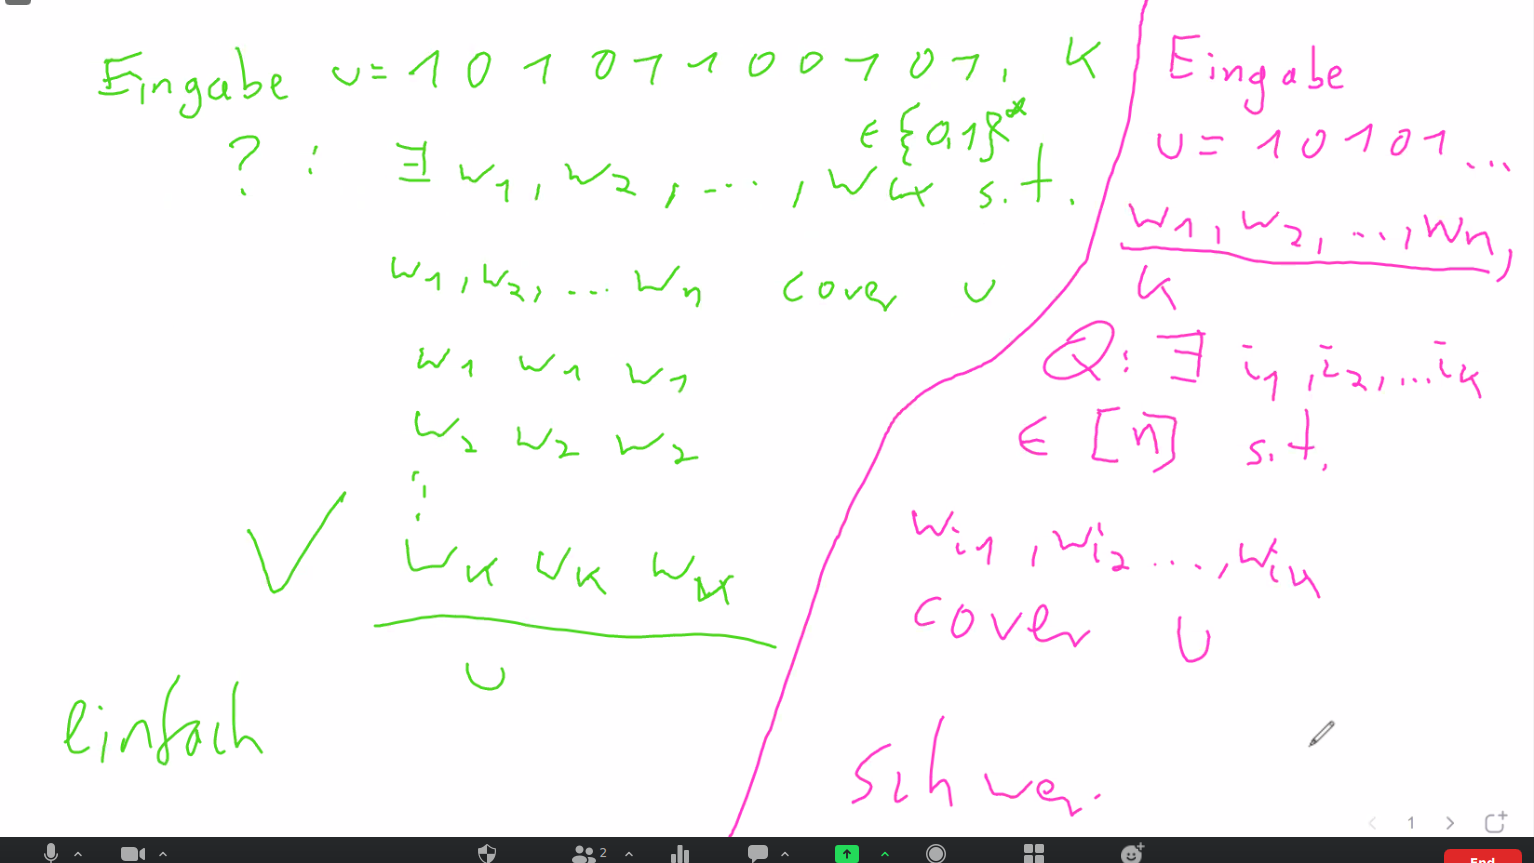
\includegraphics[width=\linewidth]{proof-sketches/Screenshot[2]-01.png}
\end{figure}

     % Analyse
%% entwurf.tex
%% $Id: entwurf.tex 61 2012-05-03 13:58:03Z bless $
%%

\chapter{Decomposition Algorithm}
\label{ch:Conceptual Design}
%% ==============================




%%% Local Variables: 
%%% mode: latex
%%% TeX-master: "thesis"
%%% End: 
     % Entwurf
%%% implemen.tex
%% $Id: implemen.tex 61 2012-05-03 13:58:03Z bless $
%%

\chapter{Implementierung}
\label{ch:Implementierung}
%% ==============================
\ldots

%% ==============================
\section{Abschnitt 1}
%% ==============================
\label{ch:Implementierung:sec:Abschnitt1}

\ldots

%% ==============================
\section{Abschnitt 2}
%% ==============================
\label{ch:Implementierung:sec:Abschnitt2}

\ldots

%%% Local Variables: 
%%% mode: latex
%%% TeX-master: "thesis"
%%% End: 
    % Implementierung
%% eval.tex
%% $Id: eval.tex 61 2012-05-03 13:58:03Z bless $

\chapter{Evaluation}
\label{ch:Evaluation}
%% ==============================

In this evaluation section, we explore how well the algorithm performs by looking at the performance and examining the decompositions. Our primary interest lies in two aspects, the size of the factors contributing to the decomposition and the coverage of final states by each factor. Through this analysis, we aim to gauge the algorithm's effectiveness in generating meaningful decompositions. This evaluation is pivotal for understanding the algorithm's capability to produce concise and relevant factors, providing insights into the temporal structure of the give labels. For this purpose, the complete f2f dataset was evaluated, described in Section \ref{ch:prelimiaries:real-world-data} consisting of 62 Temporal graphs with 20 to 56 edges each, ignoring loop edges. In total there are 3321 edges with a combined label length of around 2.3 million giving an average label length of 6993. Please not that the data sets represent people looking at each other, a directed edge from node $u$ to $v$ indicates participant $u$ looks at participant $v$ therefore only one edge label at a given time step $t$ has its value set, $\tau(e)[t] = 1$ for exactly one outgoing edged of $u$. This is also visible in the data as only 13.4\% of values in the labels is set to 1 over all the labels.

\section{Performance Evaluation}
Although performance was not the main focus of the implementation and evaluation, generating \orDecomp for the complete dataset is reasonable fast with around 3 seconds if using the maximal divisors or the greedy approach. The Fourier-transformation takes a lot of additional time for cleaning multiples of a factor as well as replacing factors with multiple set values with a set of factors with only one set value, causing it to run for 1 minute and 45 seconds. All benchmarks were performed on an AMD Ryzen 5 2600X six core processor (12 threads) with a 3.6 GHz base clock and a 4.2 GHz boost clock speed. For memory, 16GB 3200MHz ram and a Samsung evo ssd was used for persistent storage.
\begin{table}[h]
	\begin{tabular}{l|lll}
		 & MaxDivisors & GreedyShortFactors & FourierTransform  \\
		\hline
		 OR-Decomposition & 3.12 & 3.47 & 105 \\
		 AND-Decomposition & 9.85 & 24.83 & - \\
		 	
	\end{tabular}
	\caption{Decomposition time in seconds [s] for complete dataset}
	\label{tab:eval-performance}
\end{table}
It is to not that the \andDecomp is expected to be slower because of considerably greater amount of zeros in the data set as well as the modification to the cover finding algorithm. While with an \orDecomp, each additional factor can only remove outliers, in an \andDecomp an additional factor can also add new outliers. Because of that, the current outliers of a decomposition must be recalculated considering all factors. The Fourier-transform method again increases the amount of factors per cover, which hurts performance. Also it is not implemented for \andDecomp as it is not considered reasonable, since a human would still need to look at all factors since it is an \andDecomp.

\section{Decomposition Evaluation}
Moving on to the decomposition evaluation, we validate each method separately and then compare them against each other. We also benchmark \andDecomp and \orDecomp. To get an insight on how well a particular decomposition method is performing, decompose the whole data-set and then plot each factor of each decomposition by its relative size compared to the original \DFA size and the relative amount of covered values of the \DFA by this factor.
\begin{figure}[t]
	\begin{minipage}[h]{0.49\linewidth}
		\centering
		OR-decomposition
		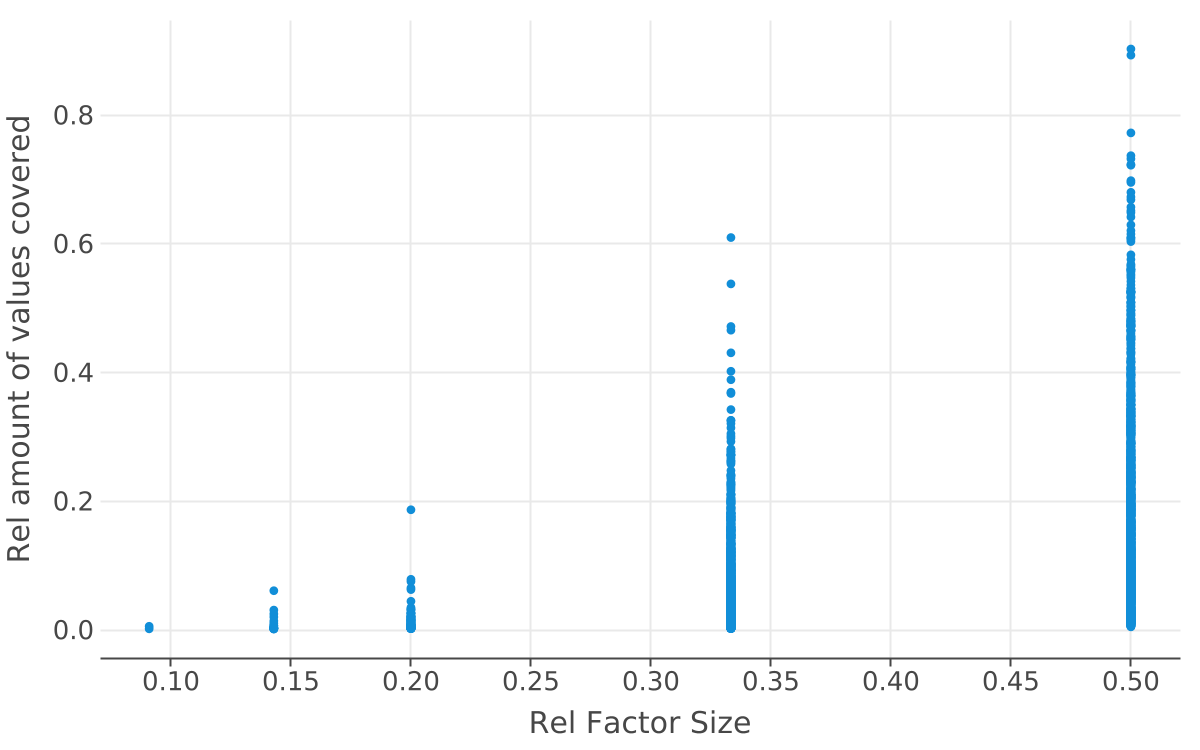
\includegraphics[width=\linewidth]{../plots/point-plots/MAX_DIVISORS-OR-all-relative-values-by-factor-size.png}
	\end{minipage}
	\begin{minipage}[h]{0.49\linewidth}
		\centering
		AND-decomposition
		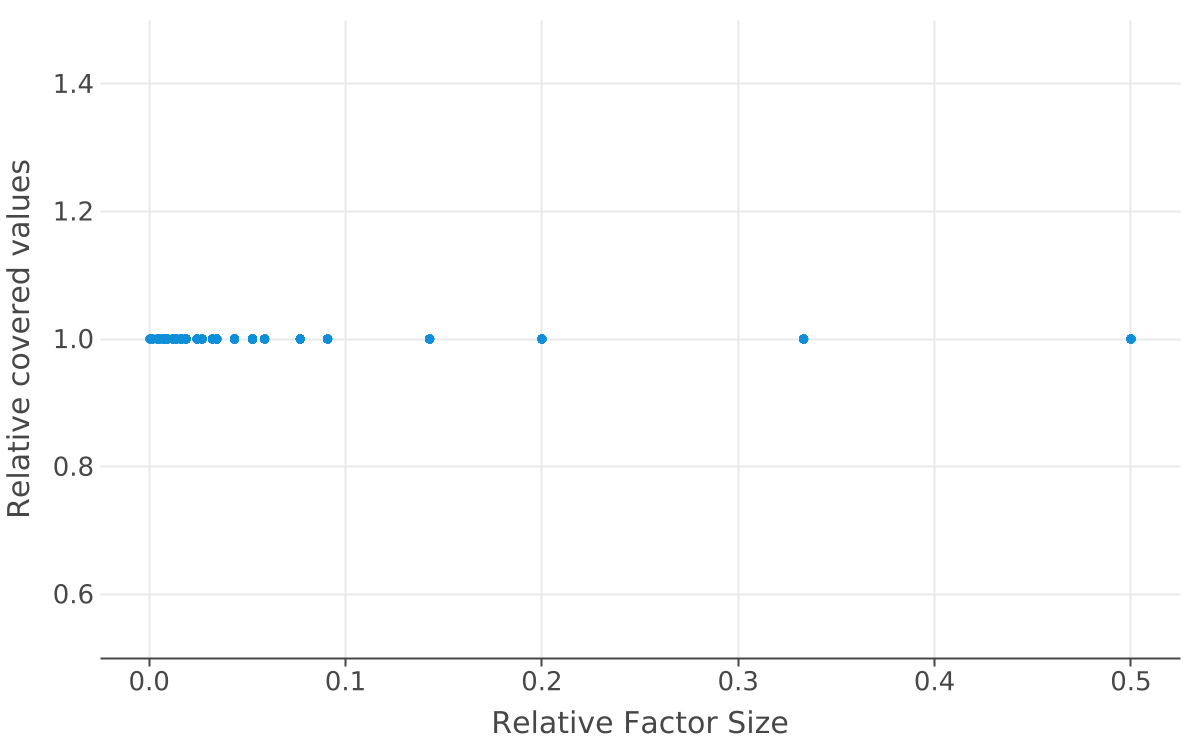
\includegraphics[width=\linewidth]{../plots/point-plots/MAX_DIVISORS-AND-all-relative-values-by-factor-size.png}
	\end{minipage}
	\caption{Relative amount of covered values by relative factor size}
	\label{fig:eval:max-divisor-all-factors}
\end{figure}

\subsection{Maximal Divisor Decomposition Evaluation}
Decomposing with the Maximal Divisor method implemented as described in Section \ref{ch:Implementation:max-divisor} was used first for decomposing the complete dataset. Analyzing the resulting decompositions and plotting each factor $B_i$ of each decomposition of a \DFA $A$ by its size relative to the original $\frac{|B_i|}{|A|}$ with its relative amount of covered final states from $A$, the precision up to that factor. The results are shown in Figure \ref{fig:eval:max-divisor-all-factors} and it clearly shows that the \orDecomp finds factors, but there are less factors in the decompositions and they cover fewer values than the comparable \andDecomp.
\begin{figure}[h]
	\begin{minipage}[h]{0.49\linewidth}
		\centering
		OR-decomposition
		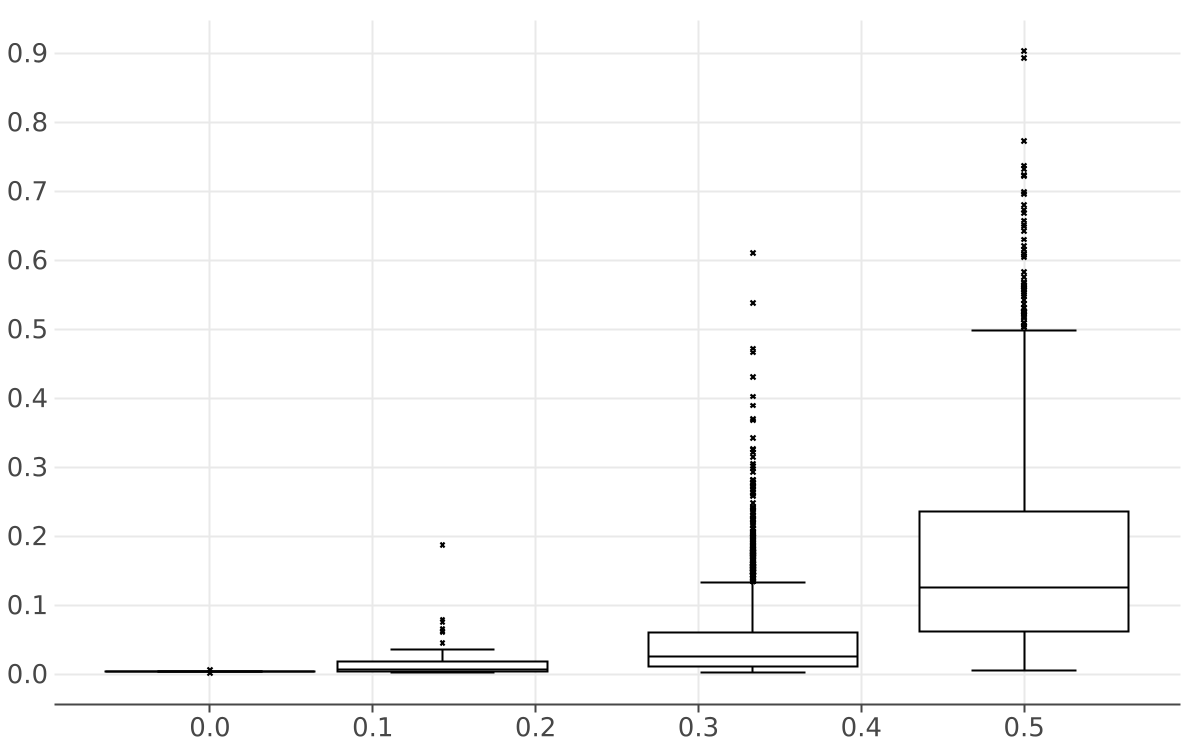
\includegraphics[width=\linewidth]{../plots/box-plots/MAX_DIVISORS-OR-all-relative-values-by-factor-boxplot-dist.png}
	\end{minipage}
	\begin{minipage}[h]{0.49\linewidth}
		\centering
		AND-decomposition
		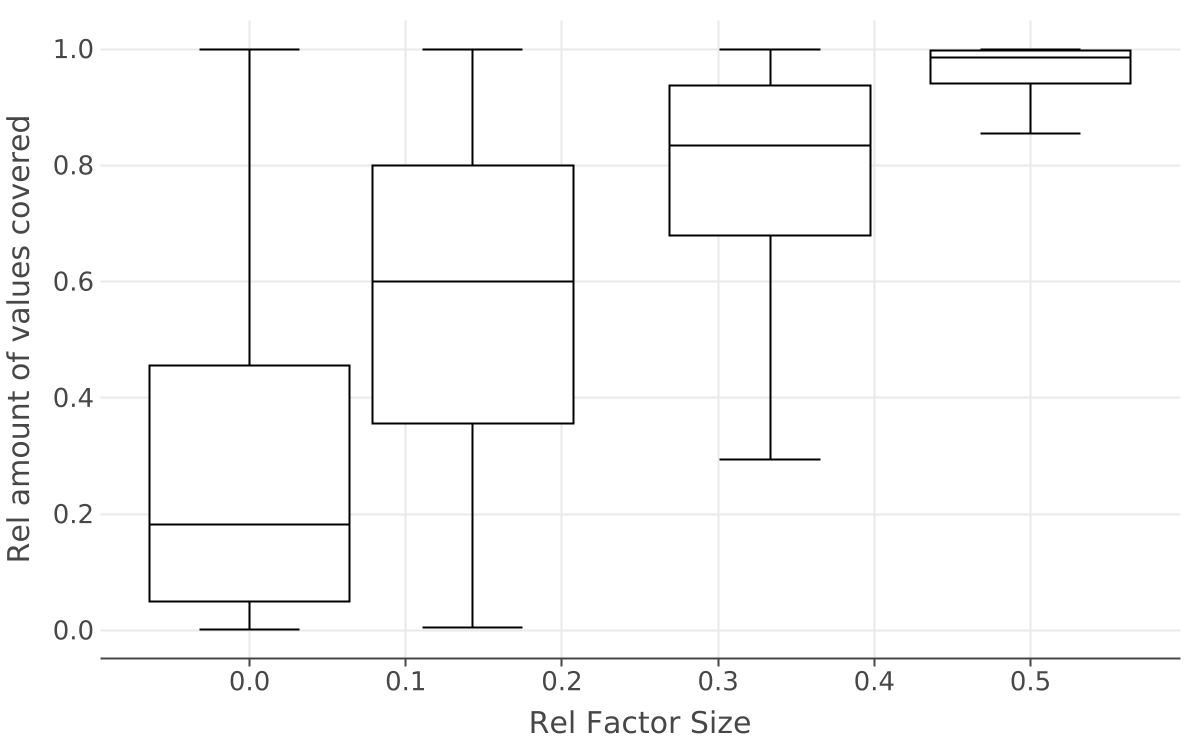
\includegraphics[width=\linewidth]{../plots/box-plots/MAX_DIVISORS-AND-all-relative-values-by-factor-boxplot-dist.png}
	\end{minipage}
	\caption{Relative amount of covered values by relative factor size (MaxDivisors)}
	\label{fig:eval:max-divisor-all-factors-box-plot}
\end{figure}
A lot of data-points collapse onto a single x value since they are grouped by their relative size, not their absolute. For the \andDecomp there are many values scattered around a small relative factor size. To get some more insight into the distribution, a box plot is also provided in Figure \ref{fig:eval:max-divisor-all-factors-box-plot}. Here, the same x and y values are chosen but the values are aggregated such that if a x value is to close to another, their data points gets merged. The \orDecomp shows that even with a relative factor size of $\frac{1}{2}$ which is the largest possible factor, the median over all these factors only cover 10\% of the target \DFA. There are some outliers with $\frac{1}{3}$ or $\frac{1}{2}$ the original size which cover already up to 60-80\% of the original \DFA but they are outliers and most of the \orDecomp found by using the maximal divisors cover almost nothing of the original, especially the short factors. For the \andDecomp a lot of the small relative factor sizes have to be aggregated in order to visualize them as box-plots, so if a relative factor size value is less than $\frac{1}{20}$ away from a previous data-point, they become one distribution. Notably, factors of size between $\frac{1}{12}$ and $\frac{1}{5}$ stretch over the entire range of relative covered values in the decomposition. With $\frac{1}{6}$ relative factor size, the \andDecomp already covered more than 50\% of a given \DFAs final states.

\subsection{Greedy Short Factor Decomposition Evaluation}
Looking at the novel greedy approach for finding short factors, a similar picture becomes evident. We find more factors and some better ones as before when using just the maximal divisors as potential factor sizes, but some factor size data points from Figure \ref{fig:eval:greedy-short-factors-all-factors} only have a single factor with that relative size. Although there are now more factors present overall, the short factors found, only cover at most 20\% of the final states of the \DFA they compose.
\begin{figure}[h]
	\begin{minipage}[h]{0.49\linewidth}
		\centering
		OR-decomposition
		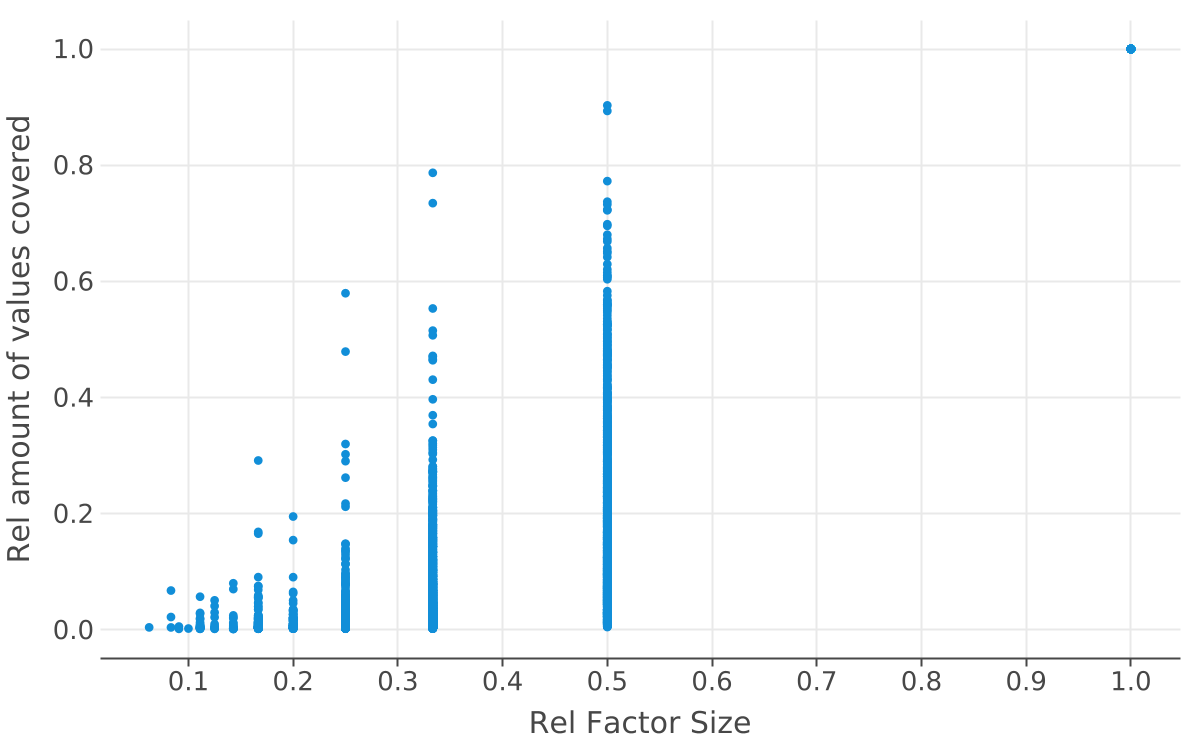
\includegraphics[width=\linewidth]{../plots/point-plots/GREEDY_SHORT_FACTORS-OR-all-relative-values-by-factor-size.png}
	\end{minipage}
	\begin{minipage}[h]{0.49\linewidth}
		\centering
		AND-decomposition
		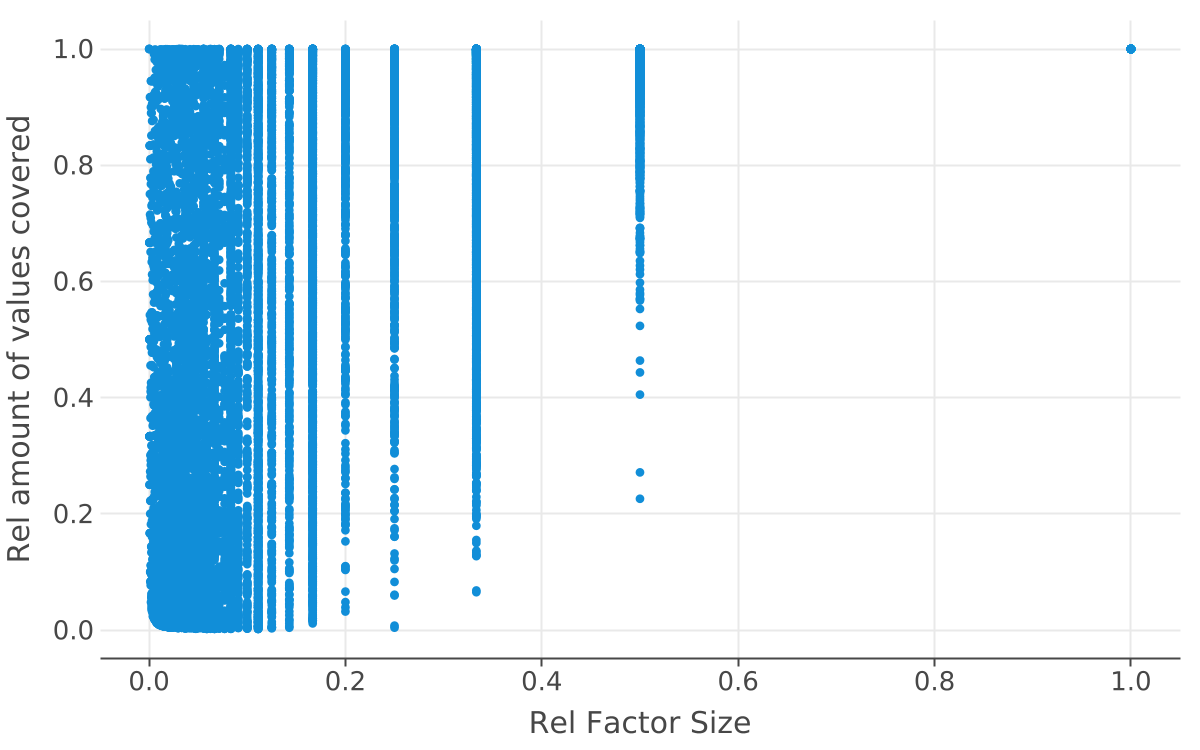
\includegraphics[width=\linewidth]{../plots/point-plots/GREEDY_SHORT_FACTORS-AND-all-relative-values-by-factor-size.png}
	\end{minipage}
	\caption{Relative amount of covered values by relative factor size}
	\label{fig:eval:greedy-short-factors-all-factors}
\end{figure}
As Figure \ref{fig:eval:greedy-short-factors-all-factors-box-plot} shows, we find more factors and even some better outliers of the distribution, but the overall covered values stays very low. There are factors of relative size $\frac{1}{3}$ or $\frac{1}{2}$ which cover up to 80\% of the final states of their \DFA present, but the median over the distributions never exceed 16\%. 
\begin{figure}[t]
	\begin{minipage}[h]{0.49\linewidth}
		\centering
		OR-decomposition
		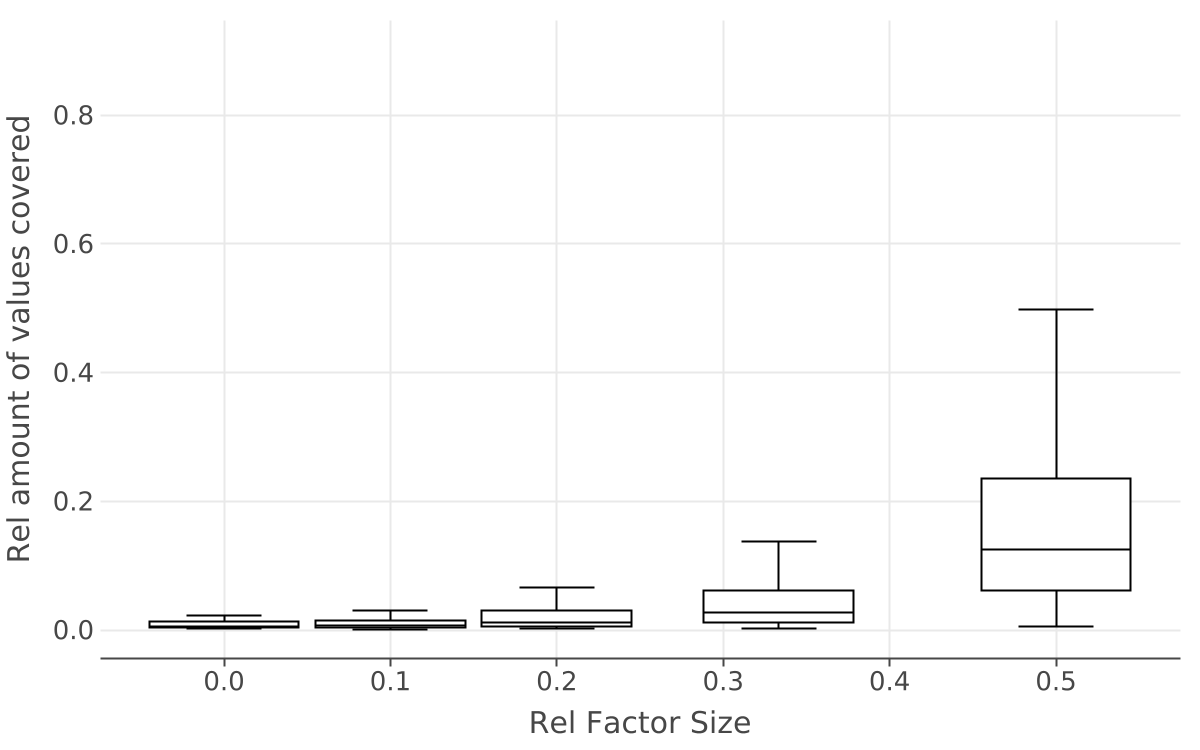
\includegraphics[width=\linewidth]{../plots/box-plots/GREEDY_SHORT_FACTORS-OR-all-relative-values-by-factor-boxplot-dist.png}
	\end{minipage}
	\begin{minipage}[h]{0.49\linewidth}
		\centering
		AND-decomposition
		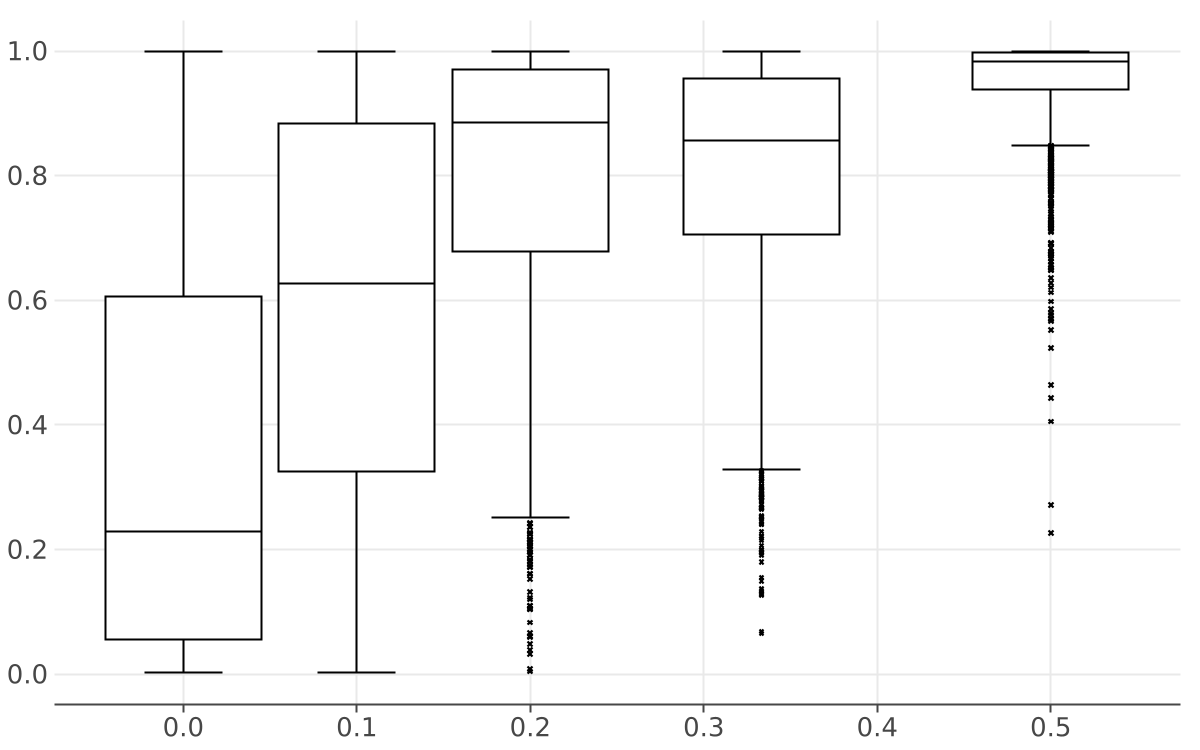
\includegraphics[width=\linewidth]{../plots/box-plots/GREEDY_SHORT_FACTORS-AND-all-relative-values-by-factor-boxplot-dist.png}
	\end{minipage}
	\caption{Relative amount of covered values by relative factor size (GreedyShorFactors)}
	\label{fig:eval:greedy-short-factors-all-factors-box-plot}
\end{figure}

TODO:elaborate

\newpage
\subsection{Fourier-Transform Decomposition Evaluation}
TODO: explain
\begin{figure}[h]
	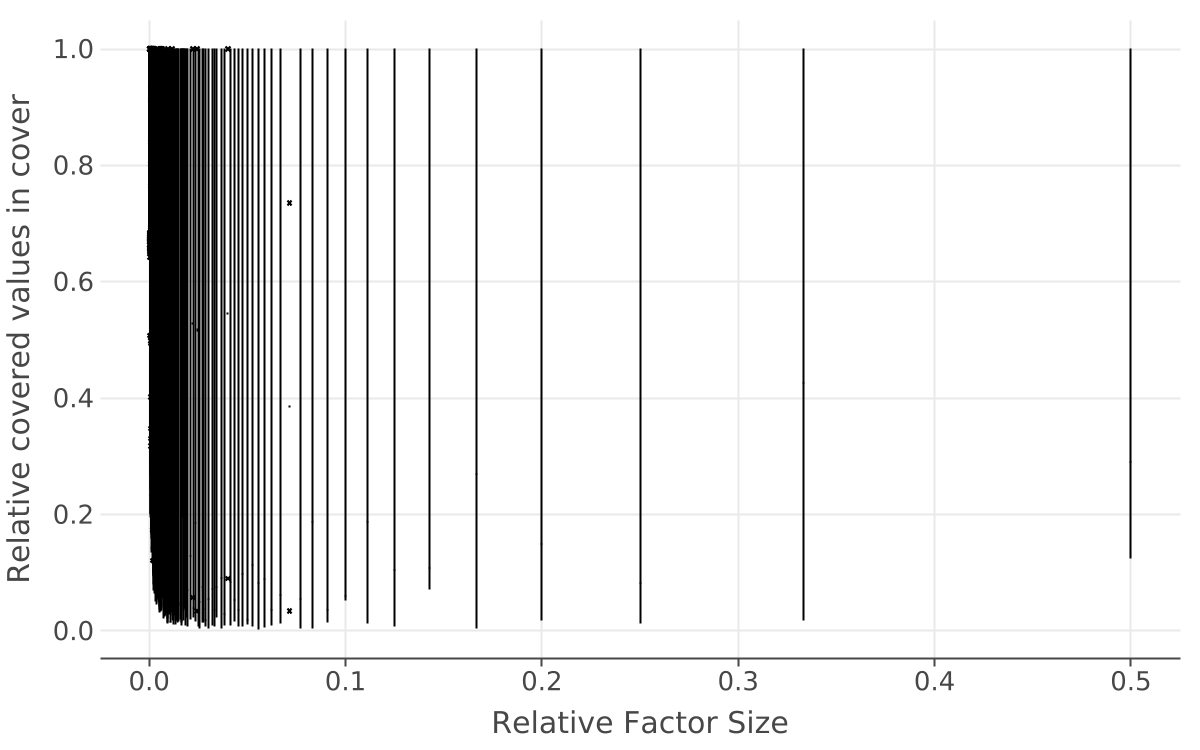
\includegraphics[width=\linewidth]{../plots/box-plots/FOURIER_TRANSFORM-OR-all-relative-values-by-factor-boxplot-outliers.png}
	\caption{Relative amount of covered values by relative factor size (FourierTransform)}
	\label{fig:eval:fourier-all-factors-box-plot}
\end{figure}

\newpage
\newpage
\section{Explainability Evaluation}
TODO: fix table, maybe remove median ? or precision in extra table as values are duplicated ?
\begin{table}[h]
	\begin{tabular}{ll||rrrrrr|rr|rrr}
		& & valid & good & ok &  \multicolumn{3}{c}{ds} & \multicolumn{2}{c}{precision} & \multicolumn{3}{c}{size}  \\
		& & & & & $\Sigma$ & a & m & avg & m & $\Sigma$ & avg & m\\
		\hline
		\hline
		\multirow{2}{*}{MaxDivisors} & $\cap$ & 182 & 1908 & 2670 & 490 & 0.14 & 0.11 &  0.86 & 0.93 & 7010 & 2.11 & 2 \\
		 & $\cup$ & 3 & 3 & 3 & 1300 & 0.39 & 0.33 & 0.08 & 0.03 & 3629 & 1.09 & 1 \\
		 \hline
		\multirow{2}{*}{GreedyShortFactors} & $\cap$ & 182 & 1908 & 2670 & 985 & 0.29 & 0.19 & 0.86 & 0.93 & 17247 & 5.19 & 3 \\
		& $\cup$ & 3 & 3 & 3 & 1396 & 0.42 & 0.33 & 0.08 & 0.03 & 4095 & 1.23 & 1 \\
		\hline
		FourierTransform & $\cup$ & 3 & 3 & 3 & 1654 & 0.49 & 0.33 & 0.08 & 0.03 & 4390 & 1.32 & 1 \\
	\end{tabular}
	\caption{Explainability metrics for different methods}
	\label{tab:eval-metric}
\end{table}

TODO: explain
%%% Local Variables: 
%%% mode: latex
%%% TeX-master: "thesis"
%%% End: 
        % Evaluation
%% zusammenf.tex
%% $Id: zusammenf.tex 61 2012-05-03 13:58:03Z bless $
%%

\chapter{Discussion}
\label{ch:Discussion}
%% ==============================
TODO:\\
- evaluate and vs or and data set\\
- contextualize evaluation\\
- outlook on explainability analysis\\

%%% Local Variables: 
%%% mode: latex
%%% TeX-master: "thesis"
%%% End: 
   	  % Diskussion und Ausblick

%% ++++++++++++++++++++++++++++++++++++++++++
%% Anhang
%% ++++++++++++++++++++++++++++++++++++++++++

\appendix
%\include{anhang_a}
%\include{anhang_b}

%% ++++++++++++++++++++++++++++++++++++++++++
%% Literatur
%% ++++++++++++++++++++++++++++++++++++++++++
%  mit dem Befehl \nocite werden auch nicht 
%  zitierte Referenzen abgedruckt

\cleardoublepage
\phantomsection
\addcontentsline{toc}{chapter}{\bibname}
%%
%%\nocite{*} % nur angeben, wenn auch nicht im Text zitierte Quellen 
           % erscheinen sollen
%\bibliographystyle{itmabbrv} % mit abgekürzten Vornamen der Autoren
\bibliographystyle{cpc} % abbrvnat unsrtnat
% spezielle Zitierstile: Labels mit vier Buchstaben und Jahreszahl
%\bibliographystyle{itmalpha}  % ausgeschriebene Vornamen der Autoren

\bibliography{thesis}

%% ++++++++++++++++++++++++++++++++++++++++++
%% Index
%% ++++++++++++++++++++++++++++++++++++++++++
\ifnotdraft{
\cleardoublepage
\phantomsection
\printindex            % Index, Stichwortverzeichnis
}

 %
 % Die folgende Erklärung ist für Diplomarbeiten Pflicht
 % (siehe Prüfungsordnung), für Studienarbeiten nicht notwendig
 \thispagestyle{empty}
%\vspace*{35\baselineskip}
%\hbox to \textwidth{\hrulefill}
\par
\chapter*{Eidesstattliche Erklärung}

Hiermit erkläre ich, dass ich diese Bachelor-/Masterarbeit selbständig verfasst und keine anderen als die angegebenen Quellen und Hilfsmittel benutzt und die aus fremden Quellen direkt oder indirekt übernommenen Gedanken als solche kenntlich gemacht habe. Die Arbeit habe ich bisher keinem anderen Prüfungsamt in gleicher oder vergleichbarer Form vor-gelegt. Sie wurde bisher auch nicht veröffentlicht.


\today

%%%%%%%%%%%%%%%%%%%%%%%%%%%%%%%%%%%%%%%%%%%%%%%%%%%%%%%%%%%%%%%%%%%%%%%%
%% Hinweis:
%%
%% Diese Erklärung wird von der Prüfungsordnung für Diplomarbeiten 
%% verlangt und ist zu unterschreiben. Für Studienarbeiten ist diese
%% Erklärung nicht zwingend notwendig, schadet aber auch nicht.
%%%%%%%%%%%%%%%%%%%%%%%%%%%%%%%%%%%%%%%%%%%%%%%%%%%%%%%%%%%%%%%%%%%%%%%%
\clearpage







 \blankpage % Leerseite auf Erklärungsrückseite
 
\end{document}
%% end of file
